\documentclass[crop,border={2pt 2pt 2pt 2pt},tikz]{standalone}
\usepackage{braket}
\usepackage{bbold}
\usepackage{bm}
\usepackage{amsmath}
\usepackage{tikz-3dplot}
% \usepackage{physics}

\usetikzlibrary{backgrounds,decorations.markings, calc}
\tikzset{>=latex}
\tikzset{->-/.style={decoration={
    markings,
    mark=at position .55 with {\arrow{>}}},postaction={decorate}}
}

\newcommand\irregularcircle[2]{% radius, irregularity
    \pgfextra {\pgfmathsetmacro\len{(#1)+rand*(#2)}}
    +(0:\len pt)
    \foreach \a in {10,20,...,350}{
        \pgfextra {\pgfmathsetmacro\len{(#1)+rand*(#2)}}
        -- +(\a:\len pt)
    }   -- cycle
}

\newcommand\irregularline[3]{% radius, irregularity
    \pgfextra {\pgfmathsetmacro\ang{(#1)+rand*(#3)}}
    +(\ang: 0)
    \foreach \a in {0,0.05,...,1}{
        \pgfextra {\pgfmathsetmacro\ang{(#1)+rand*(#3)*\a^-1}}
        -- +(\ang:{\a*(#2)})
    }  
}

\begin{document}
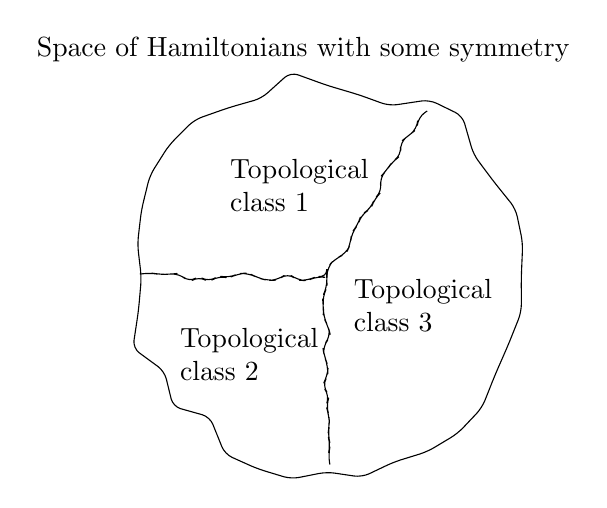
\begin{tikzpicture}[line join = round]
    \node[] at (-0.3,3.7) {Space of Hamiltonians with some symmetry};
    \coordinate (c) at (0,0.8); 
    \draw[black,rounded corners=1mm] (c) \irregularcircle{2.5cm}{2mm};
    \draw[black,rounded corners=1mm] (c) \irregularline{60}{2.6cm}{0.5mm};
    \draw[black,rounded corners=1mm] (c) \irregularline{180}{2.5cm}{0.5mm};
    \draw[black,rounded corners=1mm] (c) \irregularline{270}{2.5cm}{0.5mm};
    \node[align = left] at (100:2) {Topological \\ class 1};
    \node[align = left] at (190:1.0) {Topological \\ class 2};
    \node[align = left] at (20:1.3) {Topological \\ class 3};

\end{tikzpicture}

\end{document}